\documentclass[legalpaper]{article}
\usepackage[legalpaper, margin=1in]{geometry}
\usepackage[T1]{fontenc}
\usepackage[utf8]{inputenc}
\usepackage[italian]{babel}
\usepackage{graphicx}

\begin{document}
	\section{Progettazione logica}
		Lo scopo della progettazione logica è di costruire uno schema relazionale che rappresenti in modo accurato, efficiente e soprattutto correttamente tutte le informazioni descritte da uno schema ER prodotto durante la fase precedente. \\
		Questo non è una semplice trasformazione da un modello ad un altro per due motivi:
		\begin{itemize}
			\item non tutti i costrutti del modello ER possono essere tradotti nel modello relazionale;
			\item lo schema deve essere ristrutturato in modo che l'esecuzione delle operazioni avvenga il più efficientemente possibile
		\end{itemize}
		Inoltre si controllano e governano le ridondanze. Infatti per analizzarle si usano: 
		\begin{itemize}
			\item i volumi dei dati;
			\item operazioni attese;
			\item frequenza delle operazioni;
		\end{itemize}
		\'E utile dividere questo tipo di progettazione in due semplici step:
		\begin{itemize}
			\item ristrutturazione dello schema ER, basato sull'ottimizzazione e semplificazione dello schema;
			\item traduzione nel modello logico.
		\end{itemize}
		\begin{figure}[ht]
			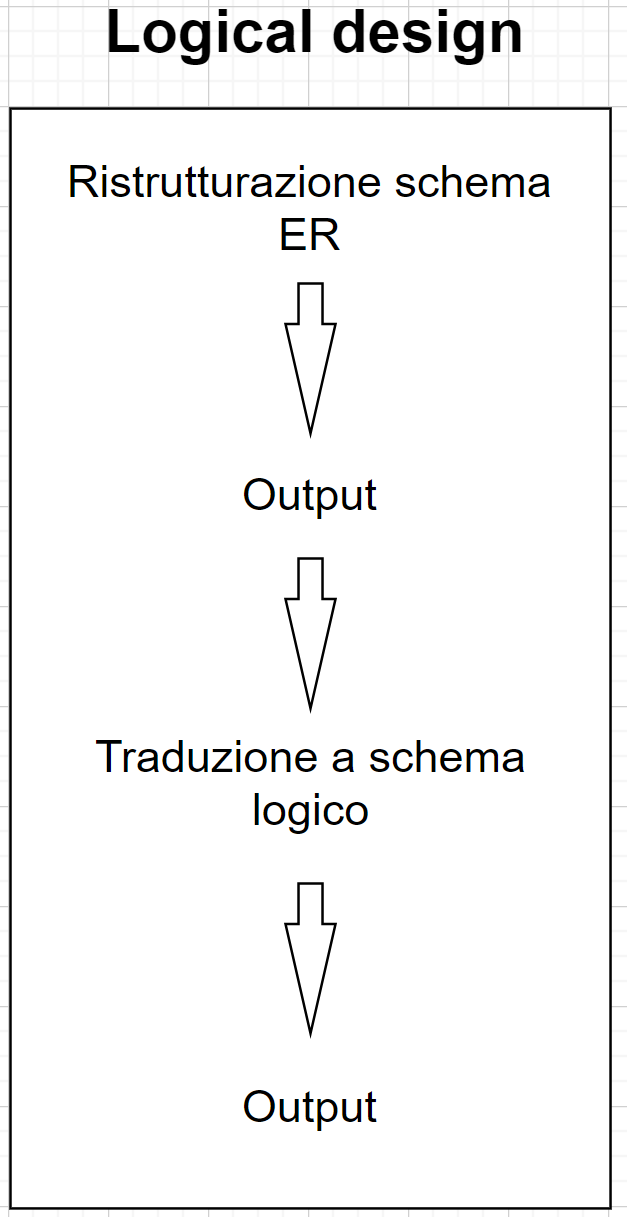
\includegraphics[width=4cm]{Schema Prog. Logica}
		\end{figure}
	\subsection{Tabella dei volumi}
		In questa sezione andiamo a definire il numero di occorrenze per ogni entità e relazione presente all'interno dello schema ER. Viene ipotizzato che i volumi facciano riferimento all'attività dopo i suoi dieci anni di vita.\\
		\newline
		\renewcommand\arraystretch{2}
		\begin{tabular}{ |p{5cm}|p{2cm}|p{5cm}| }
			\hline
			\multicolumn{3}{|c|}{\textbf{Tabella dei volumi}} \\
			\hline
			\textbf{Entità/Relazione} & \textbf{Tipo} & \textbf{Volume} \\
			\hline
			Azienda & E & ... \\ \hline
			Ente Pubblico & E & ... \\ \hline
			Persona Giuridica & E & ... \\ \hline
			Singolo Cittadino & E & ... \\ \hline
			Cliente & E & ... \\ \hline
			effettua & R & ... \\ \hline
			Richiesta & E & ... \\ \hline
			per & R & ... \\ \hline
			Assistenza & E & ... \\ \hline
			inerente & R & ... \\ \hline
			Guasto & E & ... \\ \hline
			composto da & R & ... \\ \hline
			Intervento & E & ... \\ \hline
			gestito da & R & ... \\ \hline
			è capace di risolvere & R & ... \\ \hline
			Tecnico & E & ... \\ \hline
		\end{tabular}

	
	\subsection{Tabella delle operazioni}
	Per ogni operazione indicata precedentemente, andiamo a definire la frequenza con la quale essa viene eseguita e la sua tipologia:
	\begin{itemize}
		\item \textbf{Batch}: operazioni che si possono "ignorare", ovvero vengono svolte quando il sistema non lavora in pieno regime (ad esempio tarda sera). Facendo così, si lascia spazio alle operazioni più importanti;
		\item \textbf{Interactive}: operazioni più importanti, dove la velocità di esecuzione deve essere veloce. Il tempo di risposta quindi deve essere veloce.
	\end{itemize}
		\renewcommand\arraystretch{2}
		\begin{tabular}{ |p{5cm}|p{2cm}|p{5cm}| }
			\hline
			\multicolumn{3}{|c|}{\textbf{Tabella delle operazioni}} \\
			\hline
			\textbf{Operazione} & \textbf{Tipo} & \textbf{Frequenza} \\
			\hline
			Operazione 1 & I &  media di 2 volte a settimana \\ \hline
			Operazione 2 & I & 40 volte a settimana \\ \hline
			Operazione 3 & I & 120 a settimana \\ \hline
			Operazione 4 & B & 6 volte all'anno \\ \hline
			Operazione 5 & I & 20 volte a settimana \\ \hline
			Operazione 6 & B & 1 volta a settimana \\ \hline
			Operazione 7 & B & 1 volta al mese \\ \hline
			Operazione 8 & I & 10 volte al giorno \\ \hline
			Operazione 9 & B & 1 volta al mese \\ \hline
			Operazione 10 & B & 1 volta a settimana \\ \hline
		
		\end{tabular}	
			
\end{document}